\chapter{Конструкторская часть}

В данном разделе будут рассмотрены схемы вышеизложенных алгоритмов, а также вычислена их трудоемкость.

\section{Разработка алгоритмов}

На рисунке \ref{img:bead_sort} представлен алгоритм сортировки бусинами.

\begin{figure}[H]
	\begin{center}
		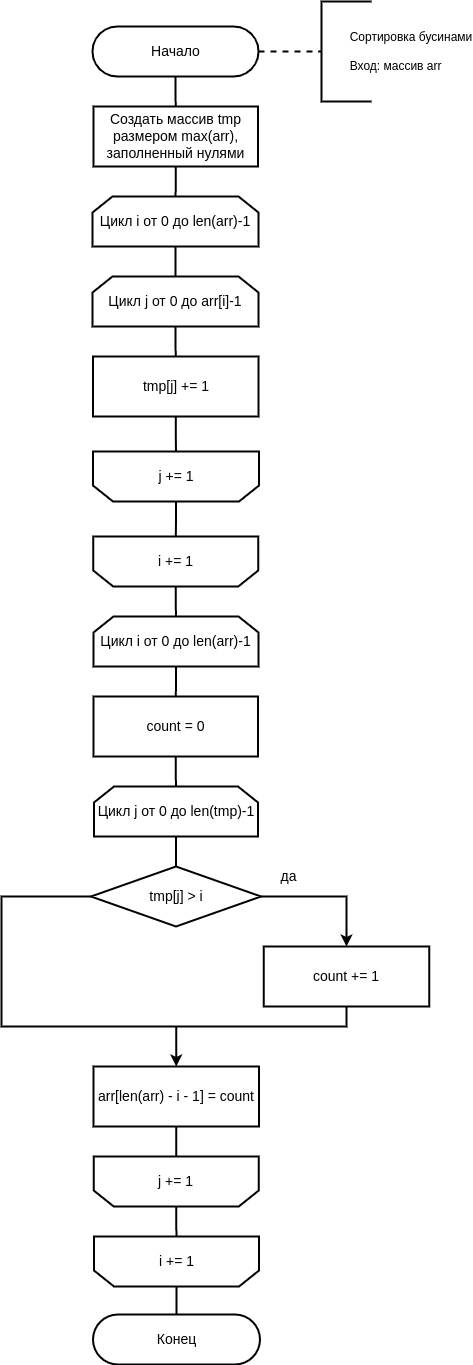
\includegraphics[scale=0.51]{img/bead_sort.png}
	\end{center}
	\captionsetup{justification=centering}
	\caption{Схема алгоритма сортировки бусинами}
	\label{img:bead_sort}
\end{figure}

На рисунке \ref{img:counting_sort} представлен алгоритм сортировки подсчетом.

\begin{figure}[H]
	\begin{center}
		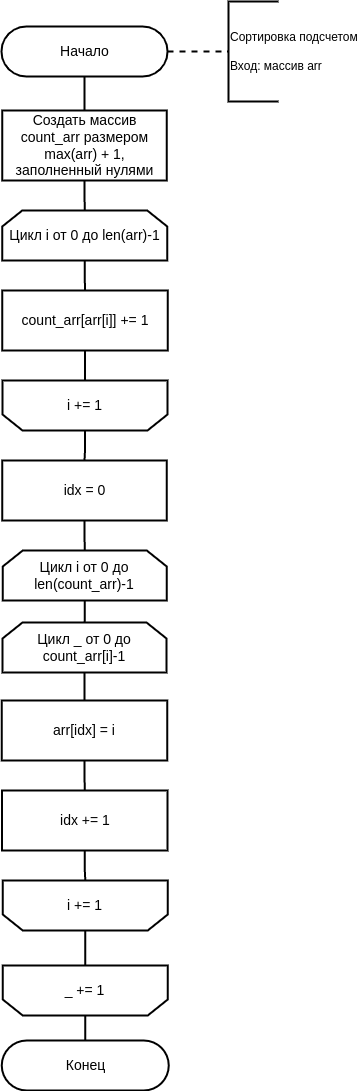
\includegraphics[scale=0.6]{img/counting_sort.png}
	\end{center}
	\captionsetup{justification=centering}
	\caption{Схема алгоритма сортировки подсчетом}
	\label{img:counting_sort}
\end{figure}

На рисунке \ref{img:gnome_sort} представлен алгоритм гномьей сортировки.

\begin{figure}[H]
	\begin{center}
		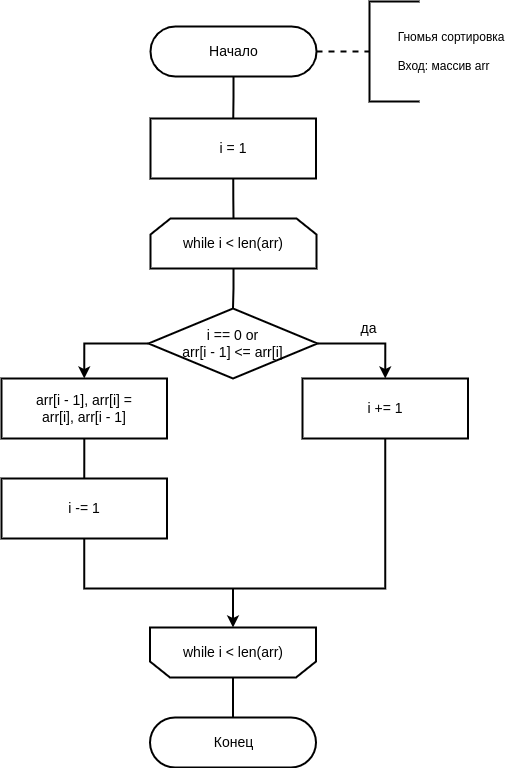
\includegraphics[scale=0.8]{img/gnome_sort.png}
	\end{center}
	\captionsetup{justification=centering}
	\caption{Схема алгоритма гномьей сортировки}
	\label{img:gnome_sort}
\end{figure}

\section{Вычислительная модель оценки трудоемкости}

\begin{enumerate}
	\item Трудоемкость следующих базовых операций равна 2:
		\begin{equation}
			/, \%, * 
		\end{equation}
	\item Трудоемкость следующих базовых операций единична:
		\begin{equation}
			=, +=, -=, ++, --, ==, !=, <, <=, >, >=, +, -, <<, >>, []
		\end{equation}
	\item Трудоемкость цикла:
	\begin{equation}
	f_{\text{цикла}} = f_{\text{иниц.}} + f_{\text{сравнения}} + N_{\text{итераций}}(f_{\text{тела}} + f_{\text{инкремент}} + f_{\text{сравнения}})
	\end{equation}
	\item Трудоемкость условного оператора:
	\begin{equation}
		f_{if} = f_{\text{выч. условия}} +
		\left[
		\begin{array}{cc}
		min(f_1, f_2), &\text{лучший случай,}\\
		max(f_1, f_2), &\text{худший случай.}
		\end{array}
		\right.
	\end{equation}
\end{enumerate}

\section{Вычисление трудоемкости алгоритмов}

\subsection{Алгоритм сортировки бусинами}

Трудоёмкость алгоритма сортировки бусинами в лучшем случае, когда массив заполнен нулями, равна $O(n)$, в худшем, когда массив запоолнен различными положительными числами, $O(S)$, где $S$ --- сумма всех чисел в массиве, $n$ --- количество элементов в массиве \cite{bead_sort}.

\subsection{Алгоритм сортировки подсчетом}

Трудоёмкость алгоритма сортировки подсчетом равна
\begin{equation}
	\label{for:counting_sort}
	\begin{array}{c}
	f_{counting\_sort} = 5 + n + 2 + n(2 + 3) + 1 + 2 + k(3 + 2) + \\(3 + 3) \cdot (n + k) = 10 + 6n + 5k + 6(n + k) \approx 6(n + k) = O(n + k),
	\end{array}
\end{equation}
где $n$ --- количество элементов в массиве, $k$ --- диапазон значений.

В лучшем случае, когда $n >> k$, трудоемкость равна $O(n)$, в худшем --- $O(n + k)$.

\subsection{Алгоритм гномьей сортировки}

Трудоёмкость алгоритма гномьей сортировки в лучшем случае, когда массив отсортирован, равна
\begin{equation}
	\label{for:gnome_sort_best}
	f_{gnome\_sort\_best} = 1 + 1 + (n - 1)(6 + 1) = 7n - 5 \approx 7n = O(n)
\end{equation}

Трудоёмкость в худшем случае, когда массив отсортирован в обратном порядке, равна (\ref{for:gnome_sort_worst}):
\begin{equation}
	\label{for:gnome_sort_worst}
	\begin{array}{c}
	f_{gnome\_sort\_worst} = 1 + 1 + (n - 1)(6 + (n - 1) \cdot (7 + 1)) =\\ 2 + (n - 1) \cdot (8n - 2) = 8n^2 - 10n + 4 \approx 8n^2 = O(n^2), 
	\end{array}
\end{equation}
где $n$ --- количество элементов в массиве.

\section*{Вывод}

На основе теоретических данных, полученных из аналитического раздела,
были построены схемы требуемых алгоритмов. Кроме того, была произведена оценка трудоемкости алгоритмов.
